% Vietnamese translation for OI Public Library
% Source-PDF: IOI中国国家候选队论文/2004/鬲融.pdf
\documentclass[11pt]{article}
\usepackage{tikz}
\usepackage{oipl-vn}

\newcommand{\BigO}{\mathcal{O}}
\newcommand{\True}{\textsf{true}}
\newcommand{\False}{\textsf{false}}

\title{Bàn về ứng dụng của tư tưởng vét cạn đặc biệt}
\author{Ge Rong\\Trường Trung học số 1 Đường Sơn, Hà Bắc}
\date{IOI 2004, đội tuyển tập huấn quốc gia Trung Quốc}

\begin{document}
\maketitle

\origtitle{Bàn về ứng dụng của tư tưởng vét cạn đặc biệt}
\sourcepath{IOI China candidate team papers / 2004 / Ge Rong.pdf}

\begin{abstract}
Bài viết phân tích một số ứng dụng đặc biệt của hai kiểu vét cạn: vét cạn
toàn phần và vét cạn từng phần. Qua các ví dụ cụ thể, bài viết cho rằng vét
cạn vẫn là một tư tưởng hữu hiệu khi giải bài, và đáng được chú ý đúng mức.
Với vét cạn toàn phần, nếu chọn đúng đối tượng cần xét, ta có thể đạt hiệu
quả mong muốn. Với vét cạn từng phần, hay phương pháp tham biến, ta có một
công cụ mạnh cho các bài toán cực tiểu hóa giá trị lớn nhất hoặc cực đại hóa
giá trị nhỏ nhất. Tư tưởng này còn mở rộng phạm vi áp dụng của các thuật toán
đồ thị, tham lam và quy hoạch động, trong khi hiệu suất thường vẫn đáp ứng
yêu cầu.
\end{abstract}

\noindent\textbf{Từ khóa:} vét cạn; vét cạn toàn phần; vét cạn từng phần;
phương pháp tham biến; bài toán cực đại--cực tiểu; ghép cực đại--cực tiểu.

\section{Mở đầu}

Vét cạn là một trong những tư tưởng quan trọng nhất của tin học. Tốc độ xử lý
cao của máy tính làm cho việc xét nhiều khả năng trở nên khả thi. Tuy nhiên,
khi lý thuyết đồ thị, số học, quy hoạch động và các thuật toán tìm kiếm ngày
càng phát triển, vét cạn dường như ngày càng ít được coi trọng, thậm chí bị
đồng nhất với ``kém hiệu quả''. Thực ra tư tưởng vét cạn vẫn có nhiều ứng
dụng. Bài viết này phân tích vài cách dùng đặc biệt của nó qua một số bài
toán tiêu biểu.

\section{Tư tưởng vét cạn}

Nói ngắn gọn, vét cạn là tư tưởng đưa ra mọi khả năng có liên quan, đôi khi
cả một số khả năng sau đó sẽ bị loại, rồi xử lý chúng. Có thể chia thành hai
dạng.

\term{Vét cạn toàn phần} xét toàn bộ không gian trạng thái đã chọn. Vì dễ sinh
ra nhiều trường hợp thừa, nó thường được thay bằng các thuật toán tìm kiếm có
cắt tỉa. Dù vậy, ta sẽ thấy vét cạn toàn phần không nhất thiết chậm hơn một
phép tìm kiếm có nhiều mẹo cắt tỉa.

\term{Vét cạn từng phần} phù hợp với các bài toán có một đại lượng quan trọng
chưa biết. Nếu biết đại lượng ấy, ta có thể giải phần còn lại bằng một thuật
toán hiệu quả. Khi đó ta chỉ xét đại lượng quan trọng này, rồi dùng thuật
toán khác để kiểm tra hoặc xây dựng lời giải.

Khi áp dụng tư tưởng vét cạn, có thể theo bốn bước:
\begin{enumerate}
  \item Hiểu chính xác đề bài. Đây là bước cần thiết với mọi phương pháp.
  \item Xác định rằng bài toán đáng dùng vét cạn. Nếu bài toán có một phương
  pháp chuyên biệt tốt hơn, nên ưu tiên phương pháp đó. Đồng thời số trạng
  thái cần xét phải đủ nhỏ để thời gian chạy chấp nhận được.
  \item Chọn rõ đối tượng cần vét cạn. Lựa chọn này ảnh hưởng trực tiếp đến
  độ phức tạp thời gian. Một đối tượng phù hợp có thể biến một lời giải tưởng
  như thô sơ thành rất hiệu quả.
  \item Giải phần còn lại của bài toán dựa trên đối tượng đã chọn.
\end{enumerate}

\subsection{Ví dụ 1: Smart Typist}

\paragraph{Đề bài.}
Cho một bàn phím đặc biệt chỉ có sáu phím: \texttt{Up}, \texttt{Down},
\texttt{Left}, \texttt{Right}, \texttt{Swap0}, \texttt{Swap1}. Vùng nhập có
sáu vị trí, đánh số từ trái sang phải là \(1,2,\ldots,6\). Phím
\texttt{Up}/\texttt{Down} tăng hoặc giảm chữ số tại vị trí con trỏ một đơn vị,
nhưng không vượt khỏi khoảng \(0\) đến \(9\). Hai phím
\texttt{Left}/\texttt{Right} di chuyển con trỏ sang trái hoặc phải. Phím
\texttt{Swap0} đổi chữ số tại con trỏ với vị trí \(1\); phím
\texttt{Swap1} đổi chữ số tại con trỏ với vị trí \(6\). Ban đầu con trỏ ở vị
trí \(1\). Cần biến một mật khẩu sáu chữ số thành một mật khẩu sáu chữ số
khác với số lần gõ ít nhất.

Ví dụ, từ trạng thái \(123456\) muốn đến \(633451\), có thể làm:
\[
123456 \xrightarrow{\texttt{Swap1}} 623451
\xrightarrow{\texttt{Right}} 623451
\xrightarrow{\texttt{Up}} 633451.
\]

\paragraph{Phân tích ban đầu.}
Sự xuất hiện của hai phím hoán đổi làm bài toán có vẻ không còn cấu trúc đơn
giản, nên cách tự nhiên là tìm kiếm trạng thái. Nhưng tổng số trạng thái cỡ
\(6\cdot 10^6\): sáu vị trí con trỏ và \(10^6\) chuỗi chữ số. Tìm kiếm trực
tiếp tốn nhiều thời gian và bộ nhớ. Có thể dùng hàm đánh giá tốt, cắt tỉa,
bảng băm kết hợp A*, hoặc BFS hai chiều, nhưng chương trình sẽ phức tạp và
hiệu suất vẫn không thật gọn.

\paragraph{Chọn đối tượng để vét cạn.}
Khó khăn nằm ở hai phím \texttt{Swap0} và \texttt{Swap1}. Nếu bỏ hai phím này
thì bài toán gần như tầm thường: chỉ cần di chuyển con trỏ và điều chỉnh từng
chữ số. Vì vậy ta xét riêng cách dùng hai phím hoán đổi.

Thoạt nhìn, việc này không khả thi: ta không biết thứ tự xen kẽ giữa các phím
hoán đổi và các phím tăng giảm, cũng không biết tổng số thao tác. Nhưng có
một nhận xét quan trọng: nếu chỉ tăng giảm cùng một chữ số, đặt thao tác
\texttt{Up}/\texttt{Down} trước hay sau thao tác hoán đổi là tương đương, miễn
là nó vẫn tác động đến chữ số tương ứng. Chẳng hạn từ \(133456\), ta có thể
dùng \texttt{Up}, \texttt{Right}, \texttt{Swap0} để thu được \(323456\); cũng
có thể dùng \texttt{Right}, \texttt{Swap0}, rồi \texttt{Up} và vẫn thu được
kết quả đó.

Do đó ta chia lời giải thành hai pha. Pha thứ nhất chỉ xét các thao tác hoán
đổi để tạo ra một hoán vị của sáu chữ số ban đầu. Pha thứ hai không còn dùng
hoán đổi, chỉ tính chi phí di chuyển và tăng giảm để đạt mật khẩu đích. Số
hoán vị của sáu vị trí chỉ là \(6!=720\), nên có thể dùng vét cạn hoặc BFS
trên không gian hoán vị để tính số thao tác hoán đổi nhỏ nhất.

Vẫn còn một chi tiết: trong quá trình tạo một hoán vị, con trỏ có thể chưa
đi qua mọi vị trí, nên không phải vị trí nào cũng có thể được điều chỉnh
không tốn thêm thao tác \texttt{Left}/\texttt{Right}. Nếu xét trạng thái ``vị
trí nào đã có thể chỉnh'', có tối đa \(2^6=64\) khả năng, vẫn chỉ tạo
\(720\cdot 64=46080\) trạng thái, bằng khoảng \(0.77\%\) không gian tìm kiếm
trực tiếp.

Phân tích kỹ hơn còn giảm được nữa:
\begin{enumerate}
  \item Vị trí \(1\) luôn có thể chỉnh, vì con trỏ xuất phát tại đó.
  \item Với các vị trí \(2,3,4,5\), nếu một vị trí bên phải đã có thể chỉnh
  thì mọi vị trí bên trái của nó cũng có thể chỉnh trong quá trình đi qua.
  Vì vậy tập các vị trí chỉnh được trong đoạn này chỉ có năm dạng:
  \[
    \varnothing,\ \{2\},\ \{2,3\},\ \{2,3,4\},\ \{2,3,4,5\}.
  \]
  \item Vị trí \(6\) có thể chỉnh hoặc chưa, tùy việc có dùng \texttt{Swap1}
  hay chưa.
\end{enumerate}
Tổng cộng chỉ có \(2\cdot 5=10\) dạng phụ, tức khoảng \(7200\) trạng thái.
Đây là điểm then chốt: chọn đúng đối tượng vét cạn làm bài toán trở nên nhỏ
và dễ cài đặt.

\begin{center}
\begin{tabular}{llll}
\textbf{Thuật toán} & \textbf{Độ phức tạp} & \textbf{Cài đặt} & \textbf{Nhận xét}\\
\hline
Tìm kiếm trạng thái & rất lớn & khó & chưa tận dụng điều kiện đề\\
Vét cạn đã chọn & \(\BigO(720\cdot 10)\) & khá nhỏ & khai thác cấu trúc hoán đổi
\end{tabular}
\end{center}

\subsection{Ví dụ 2: Logic Island}

\paragraph{Đề bài.}
Trên Logic Island có ba loại cư dân: thần luôn nói thật, ác quỷ luôn nói dối,
và người thường nói thật vào ban ngày nhưng nói dối vào ban đêm. Một nhà xã
hội học đến thăm đảo, nhưng không thể phân biệt loại cư dân bằng vẻ ngoài.
Trên đảo chỉ có năm cư dân \(A,B,C,D,E\). Mỗi câu nói thuộc một trong ba dạng:
\begin{enumerate}
  \item \texttt{I am [not] divine/evil/human/lying.}
  \item \texttt{X is [not] divine/evil/human/lying.}
  \item \texttt{It is day/night.}
\end{enumerate}
Tổng số câu không quá \(50\). Cần suy ra loại của từng cư dân và thời điểm là
ban ngày hay ban đêm, nếu các dữ kiện cho phép.

Xét ví dụ:
\begin{verbatim}
A: B is human.
B: A is evil.
A: B is evil.
\end{verbatim}
Nếu suy luận bằng tay, hai câu của \(A\) mâu thuẫn nhau, nên \(A\) đang nói
dối. Khi đó \(B\) không thể là người hay ác quỷ trong cấu hình này; \(B\) là
thần, và vì thần nói thật nên \(A\) là ác quỷ. Kết luận là:
\begin{verbatim}
A is evil.
B is divine.
\end{verbatim}

\paragraph{Áp dụng vét cạn.}
Nếu cố mô phỏng kiểu suy luận trên bằng chương trình, các nhánh suy luận khá
rối. Nhưng số cư dân chỉ là \(5\), mỗi người có \(3\) loại, còn thời gian chỉ
có hai khả năng. Tổng số giả thiết là
\[
  3^5\cdot 2=486.
\]
Đây là đối tượng vét cạn tự nhiên. Với mỗi giả thiết, ta kiểm tra từng câu
nói có phù hợp với loại của người nói và thời điểm hay không. Những giả thiết
phù hợp được giữ lại. Một sự kiện được xem là suy ra chắc chắn nếu nó đúng
trong mọi giả thiết còn lại; nếu không có giả thiết nào thì cuộc hội thoại là
bất khả.

\subsection{Tiểu kết}

Hai ví dụ trên cho thấy vét cạn toàn phần có vẻ mù quáng, nhưng người thiết
kế thuật toán thì không. Phân tích đề bài đủ sâu và chọn linh hoạt đối tượng
cần xét có thể biến một bài toán khó thành một bài toán nhỏ, giảm độ phức tạp
cài đặt và vẫn đạt hiệu quả tốt.

\section{Vét cạn từng phần: phương pháp tham biến}

Các phương pháp như đồ thị, tham lam và quy hoạch động đã rất phát triển,
nhưng bản thân chúng vẫn có giới hạn. Nhiều bài toán chỉ vì một điều kiện
khó chịu mà ta không áp dụng được thuật toán hiệu quả quen thuộc. Vét cạn
từng phần là một cách phá giới hạn ấy.

Phương pháp tham biến hoạt động như sau. Trước hết ta xét một kết quả quan
trọng của bài toán như một tham biến. Sau đó dùng tham lam, quy hoạch động,
đồ thị hoặc một công cụ khác để kiểm tra tham biến đó có khả thi hay không,
đồng thời suy ra những thành phần còn lại của lời giải.

\[
\begin{array}{c}
\text{không gian lời giải đầy đủ, quá lớn để xét trực tiếp}\\[0.5em]
\Downarrow\\[0.5em]
\text{chọn một kết quả quan trọng làm tham biến}\\[0.5em]
\Downarrow\\[0.5em]
\text{xét tham biến và kiểm tra khả thi bằng thuật toán hiệu quả}\\[0.5em]
\Downarrow\\[0.5em]
\text{xây dựng các kết quả còn lại}
\end{array}
\]

Vì chỉ xét tham biến quan trọng, còn phần khác được xử lý bằng thuật toán
hiệu quả, độ phức tạp thường là đa thức. Đôi khi vẫn cần tận dụng thêm tính
chất riêng của đề để tối ưu.

Tính chất quan trọng nhất thường là \term{đơn điệu}. Nếu tham biến \(x_1\)
khả thi thì mọi \(x\ge x_1\) cũng khả thi, và bài toán yêu cầu giá trị nhỏ
nhất của tham biến, ta có hai lựa chọn:
\begin{enumerate}
  \item xét tuyến tính và dừng ở nghiệm khả thi đầu tiên;
  \item xét bằng chia đôi.
\end{enumerate}
Chia đôi bảo đảm độ phức tạp thấp hơn, nhưng cài đặt phức tạp hơn một chút.
Với miền giá trị nhỏ, hoặc khi nghiệm thường nằm gần biên, cách tuyến tính có
thể tiết kiệm thời gian lập trình và giảm lỗi. Dù chia đôi không duyệt từng
giá trị một, tư tưởng của nó vẫn thống nhất với vét cạn từng phần.

Nhìn chung, các bài toán cực tiểu hóa giá trị lớn nhất hoặc cực đại hóa giá
trị nhỏ nhất rất hợp với phương pháp này. Chẳng hạn bài toán định nghĩa một
trọng số và yêu cầu tạo một phân hoạch sao cho trọng số lớn nhất của mỗi phần
được nhỏ nhất. Ta thường chuyển thành: đã biết một ngưỡng \(x\), có tồn tại
một phân hoạch thỏa yêu cầu hay không? Bài toán kiểm tra này là điểm mấu chốt:
nó phải đúng, dựng được nghiệm khi cần, và đủ nhanh vì có thể bị gọi nhiều
lần.

\subsection{Ví dụ 3: Strawberry}

\paragraph{Đề bài.}
Các tinh linh trong rừng muốn chia một ruộng dâu thành \(k\) mảnh và trồng
vào \(k\) khoảng đất trống. Mỗi mảnh phải liên thông theo các tua nối giữa
các cây dâu. Nếu một mảnh có tổng khối lượng quá nhỏ thì các cây dâu sẽ cô
đơn, nên các tinh linh muốn mảnh nhẹ nhất càng nặng càng tốt.

Ký hiệu \(\mathrm{sum}_i\) là tổng khối lượng dâu trong mảnh thứ \(i\), với
\(1\le i\le k\). Đặt
\[
  x=\min\{\mathrm{sum}_i\mid 1\le i\le k\}.
\]
Cần chia ruộng dâu thành \(k\) mảnh liên thông sao cho \(x\) lớn nhất, rồi
in phương án và giá trị \(x\).

Bản gốc là một bài nộp đáp án. Nhiều dữ liệu của bài có dạng cây; ở đây ta
xét trường hợp cấu trúc là cây và cần nghiệm tối ưu.

\paragraph{Phân tích ban đầu.}
Khi gặp bài toán tối ưu trên cây, ta dễ nghĩ đến quy hoạch động. Gọi
\(D(v,k)\) là giá trị tốt nhất khi chia cây con gốc \(v\) thành \(k\) phần.
Nếu \(v\) có các con \(c_1,\ldots,c_t\), một công thức tự nhiên là xét mọi
cách tách
\[
  k=a_1+a_2+\cdots+a_t
\]
rồi kết hợp các giá trị
\[
  D(c_1,a_1),D(c_2,a_2),\ldots,D(c_t,a_t),
\]
kèm điều chỉnh do gán đỉnh \(v\) vào một phần nào đó. Vấn đề nằm ở phần điều
chỉnh này: để biết sau khi thêm \(v\) thì mảnh nhỏ nhất thay đổi thế nào, ta
không chỉ cần giá trị nhỏ nhất mà còn có thể cần giá trị nhỏ thứ hai, rồi thứ
ba, và cuối cùng gần như phải lưu mọi khả năng. Công thức tuy có vẻ đúng
nhưng không khả thi về thời gian và bộ nhớ.

\paragraph{Chọn tham biến.}
Giả sử đã biết một giá trị \(x\). Ta hỏi: có thể chia cây thành ít nhất \(k\)
mảnh liên thông, mỗi mảnh có tổng khối lượng ít nhất \(x\), hay không? Nếu
trả lời được câu hỏi này, ta có thể xét các giá trị \(x\) và tìm giá trị lớn
nhất khả thi.

Câu hỏi kiểm tra thực ra không khó. Duyệt cây từ dưới lên. Với mỗi đỉnh \(v\):
\begin{itemize}
  \item \(T(v)\) là số mảnh đã tách được trong cây con của \(v\), mỗi mảnh có
  khối lượng ít nhất \(x\);
  \item \(L(v)\) là khối lượng còn dư lớn nhất chưa tách thành mảnh sau khi
  đã đạt \(T(v)\).
\end{itemize}
Gọi \(w(v)\) là khối lượng của \(v\), và các con của \(v\) là
\(c_1,\ldots,c_t\). Đặt
\[
  R=w(v)+\sum_{i=1}^{t}L(c_i).
\]
Nếu \(R\ge x\), ta tách thêm một mảnh chứa \(v\) và các phần dư từ con:
\[
  T(v)=1+\sum_{i=1}^{t}T(c_i),\qquad L(v)=0.
\]
Nếu \(R<x\), ta chưa tách được mảnh mới:
\[
  T(v)=\sum_{i=1}^{t}T(c_i),\qquad L(v)=R.
\]

Đây có thể xem là quy hoạch động, cũng có thể xem là tham lam: xử lý từ lá
lên gốc, gặp nơi đủ khối lượng thì cắt ngay. Quy hoạch động cho chứng minh
đúng khá rõ; kết quả tham lam trùng với quy hoạch động nên thuật toán tham
lam cũng đúng.

Vì tính khả thi đơn điệu theo \(x\): nếu chia được với ngưỡng \(x\) thì cũng
chia được với mọi ngưỡng nhỏ hơn, ta dùng chia đôi trên \(x\). Mỗi lần kiểm
tra mất \(\BigO(n)\) trên cây, nên tổng thời gian là
\(\BigO(n\log W)\), với \(W\) là tổng khối lượng.

\subsection{Ghép cực đại--cực tiểu}

Vét cạn từng phần cũng xuất hiện trong các thuật toán kinh điển. Một ví dụ
quan trọng là ghép hoàn hảo trong đồ thị hai phía có trọng số, tối ưu theo
ngưỡng biên.

\paragraph{Bài toán.}
Cho một đồ thị hai phía có trọng số. Cần tìm một ghép hoàn hảo sao cho trọng
số lớn nhất trong các cạnh được chọn là nhỏ nhất. Nếu đặt
\[
  x=\max\{w(e)\mid e\ \text{là cạnh được chọn}\},
\]
ta cần cực tiểu hóa \(x\).

\paragraph{Phân tích.}
Bài toán không chuyển trực tiếp thành ghép cực đại hay ghép trọng số cực đại
quen thuộc. Mô hình luồng mạng thông thường cũng không khớp ngay, vì thông
tin cần tối ưu là một giá trị biên, không phải tổng trọng số cộng được.

Nếu biết một ngưỡng \(x\), bài toán kiểm tra trở nên đơn giản: chỉ giữ những
cạnh có trọng số không vượt quá \(x\). Ta thu được một đồ thị hai phía không
trọng số. Nếu trong đồ thị này tồn tại ghép hoàn hảo thì có một nghiệm có
giá trị biên không vượt quá \(x\); ngược lại, ngưỡng \(x\) không đủ.

Về cách xét \(x\), miền trọng số có thể rất lớn, nhưng các giá trị có hiệu
lực chỉ là trọng số của các cạnh, nhiều nhất \(n^2\) giá trị với đồ thị đầy
đủ \(n\times n\). Có thể sắp xếp các trọng số rồi xét tuyến tính; để ổn định
hơn về thời gian, thường dùng chia đôi trên danh sách trọng số đã sắp xếp.

Cùng một khuôn mẫu còn xử lý được biến thể đối xứng: tìm ghép hoàn hảo sao
cho trọng số nhỏ nhất trong các cạnh được chọn là lớn nhất. Khi đó kiểm tra
ngưỡng \(x\) bằng cách giữ các cạnh có trọng số ít nhất \(x\), rồi tìm ghép
hoàn hảo.

\section{Kết luận}

Bài viết dùng vét cạn toàn phần và vét cạn từng phần để xử lý một số bài
toán. Từ các ví dụ có thể thấy:
\[
  \text{vét cạn} \ne \text{kém hiệu quả}.
\]
Với vét cạn toàn phần, việc chọn đúng đối tượng quyết định hiệu quả. Với vét
cạn từng phần, phương pháp tham biến là công cụ mạnh cho các bài toán cực
trị dạng biên, đồng thời mở rộng phạm vi áp dụng của đồ thị, tham lam và quy
hoạch động.

\begin{center}
\begin{tabular}{lll}
\textbf{Tiêu chí} & \textbf{Vét cạn toàn phần} & \textbf{Vét cạn từng phần}\\
\hline
Thời gian & phụ thuộc mạnh vào đối tượng & thường khá tốt\\
Bộ nhớ & thường tốt & phụ thuộc thuật toán kiểm tra\\
Cài đặt & tương đối thấp & phụ thuộc thuật toán kiểm tra\\
Điểm khó & chọn đối tượng & chọn tham biến\\
Phạm vi & khi thiếu phương pháp chuyên biệt & bài toán cực trị dạng biên\\
\end{tabular}
\end{center}

Tóm lại, cả vét cạn toàn phần và vét cạn từng phần đều là tư tưởng hữu hiệu
trong giải bài. Ta nên lựa chọn theo tính chất cụ thể của đề, thay vì mặc
định loại bỏ vì cho rằng mọi phương pháp vét cạn đều chậm.

\section*{Tài liệu tham khảo}

\begin{enumerate}
  \item Yu Wei, báo cáo lời giải NOI 2001.
  \item Wu Wenhu và Wang Jiande, \textit{Thuật toán và lập trình đồ thị},
  Nhà xuất bản Đại học Thanh Hoa.
\end{enumerate}

\appendix
\section{Phụ lục: đề bài và chương trình gốc}

Bản gốc kèm bốn chương trình Pascal dài. Theo ngoại lệ không dịch mẫu mã nguồn
của dự án, phụ lục này dịch đầy đủ các đề bài, dữ liệu mẫu và ghi chú chấm
điểm; phần chương trình được thay bằng tóm tắt thuật toán tương ứng.

\subsection{Bài 1: Smart Typist}

\begin{center}
\textbf{Smart Typist}\\
\texttt{clever.pas/c/cpp}
\end{center}

Alan là nhân viên đánh máy của một bộ phận cơ mật. Cô nhận nhiệm vụ trong một
ngày phải nhập vài trăm mật khẩu có độ dài cố định là \(6\). Tất nhiên, cô
muốn tổng số lần gõ phím càng ít càng tốt.

Do yêu cầu bảo mật, bàn phím dùng để nhập mật khẩu được thiết kế đặc biệt:
không có phím số, chỉ có sáu phím \texttt{Swap0}, \texttt{Swap1},
\texttt{Up}, \texttt{Down}, \texttt{Left}, \texttt{Right}. Vùng nhập có sáu
vị trí, đánh số từ trái sang phải là \(1,2,3,4,5,6\). Tác dụng của các phím:
\begin{itemize}
  \item \texttt{Swap0}: con trỏ không đổi; đổi chữ số tại con trỏ với chữ số ở
  vị trí \(1\). Nếu con trỏ đang ở vị trí \(1\), vùng nhập không đổi.
  \item \texttt{Swap1}: con trỏ không đổi; đổi chữ số tại con trỏ với chữ số ở
  vị trí \(6\). Nếu con trỏ đang ở vị trí \(6\), vùng nhập không đổi.
  \item \texttt{Up}: con trỏ không đổi; tăng chữ số tại con trỏ thêm \(1\),
  trừ khi chữ số đó đã là \(9\).
  \item \texttt{Down}: con trỏ không đổi; giảm chữ số tại con trỏ đi \(1\),
  trừ khi chữ số đó đã là \(0\).
  \item \texttt{Left}: đưa con trỏ sang trái một vị trí; nếu con trỏ đã ở vị
  trí \(1\), con trỏ không đổi.
  \item \texttt{Right}: đưa con trỏ sang phải một vị trí; nếu con trỏ đã ở vị
  trí \(6\), con trỏ không đổi.
\end{itemize}

Trước mỗi lần nhập mật khẩu, vùng nhập ngẫu nhiên xuất hiện một mật khẩu ban
đầu độ dài \(6\), và con trỏ luôn đặt ở vị trí \(1\). Sau khi dùng khéo léo
sáu phím trên, ta cần thu được mật khẩu đích; khi kết thúc con trỏ được phép
dừng ở bất kỳ vị trí nào. Hãy viết chương trình tính số lần gõ ít nhất để
nhập một mật khẩu.

\paragraph{Dữ liệu vào \texttt{clever.in}.}
Tệp chỉ có một dòng, gồm hai số độ dài \(6\): mật khẩu ban đầu và mật khẩu
đích, cách nhau bởi một dấu cách.

\paragraph{Dữ liệu ra \texttt{clever.out}.}
Tệp chỉ có một dòng, gồm một số nguyên dương là số lần gõ phím ít nhất.

\begin{verbatim}
Input
123456 654321

Output
11
\end{verbatim}

Một dãy phím đạt số lần gõ nhỏ nhất là:
\begin{center}
\begin{tabular}{ll}
\textbf{Phím} & \textbf{Vùng nhập sau khi gõ}\\
\hline
ban đầu & \texttt{123456}\\
\texttt{Swap1} & \texttt{623451}\\
\texttt{Right} & \texttt{623451}\\
\texttt{Swap0} & \texttt{263451}\\
\texttt{Down} & \texttt{253451}\\
\texttt{Right} & \texttt{253451}\\
\texttt{Up} & \texttt{254451}\\
\texttt{Right} & \texttt{254451}\\
\texttt{Down} & \texttt{254351}\\
\texttt{Right} & \texttt{254351}\\
\texttt{Up} & \texttt{254361}\\
\texttt{Swap0} & \texttt{654321}
\end{tabular}
\end{center}

Chương trình gốc chỉ vét cạn một phần tình huống dùng \texttt{Swap0}/
\texttt{Swap1} nhưng vẫn qua mọi dữ liệu; bản thân chú thích gốc nói rằng vét
cạn hoàn chỉnh nên dùng BFS trước để sinh các trạng thái hoán vị. Ý tưởng là
xét chuỗi hoán đổi, áp dụng nó lên mật khẩu ban đầu, rồi cộng số lần chỉnh
chữ số và chi phí di chuyển con trỏ.

\subsection{Bài 2: Logic Island}

Trên Logic Island có ba loại cư dân: thần luôn nói thật, ác quỷ luôn nói dối,
và người thường nói thật vào ban ngày nhưng nói dối vào ban đêm. Mọi cư dân
đều biết loại của mọi cư dân khác.

Một nhà xã hội học muốn đến đảo. Vì không thể phân biệt ba loại cư dân bằng
ngoại hình, ông cần một bộ phân tích hội thoại để suy ra các sự kiện từ lời
nói của cư dân. Các sự kiện cần biết là hiện tại ngày hay đêm, và từng người
nói thuộc loại nào.

\paragraph{Dữ liệu vào.}
Dữ liệu gồm nhiều mô tả hội thoại. Mỗi mô tả bắt đầu bằng số nguyên \(n\), số
câu nói trong hội thoại. Tiếp theo là \(n\) dòng, mỗi dòng là một câu nói của
một cư dân. Dòng câu nói bắt đầu bằng tên người nói, là một trong các chữ cái
in hoa \texttt{A}, \texttt{B}, \texttt{C}, \texttt{D}, \texttt{E}, tiếp theo là
dấu hai chấm. Phần còn lại thuộc một trong các dạng:
\begin{verbatim}
I am [not] ( divine | human | evil | lying ).
X is [not] ( divine | human | evil | lying ).
It is ( day | night ).
\end{verbatim}
Dấu ngoặc vuông nghĩa là từ trong ngoặc có thể xuất hiện hoặc không; dấu ngoặc
tròn nghĩa là chọn đúng một trong các phương án phân tách bởi dấu \texttt{|}.
\texttt{X} là một tên trong \texttt{A}, \texttt{B}, \texttt{C}, \texttt{D},
\texttt{E}. Trong một dòng không có hai dấu cách liên tiếp, và mỗi hội thoại có
nhiều nhất \(50\) câu. Dữ liệu kết thúc bằng một test có \(n=0\).

\paragraph{Dữ liệu ra.}
Với mỗi hội thoại, trước hết in số thứ tự hội thoại theo dạng trong mẫu. Nếu
hội thoại không thể xảy ra theo các quy tắc, in:
\begin{verbatim}
This is impossible.
\end{verbatim}
Nếu không suy ra được sự kiện chắc chắn nào, in:
\begin{verbatim}
No facts are deducible.
\end{verbatim}
Ngược lại, in mọi sự kiện suy ra được. Các sự kiện có dạng:
\begin{verbatim}
X is ( divine | human | evil ).
It is ( day | night ).
\end{verbatim}
Các sự kiện về cư dân phải in trước, theo thứ tự chữ cái; sau đó mới in sự
kiện ngày/đêm nếu suy ra được. Sau mỗi hội thoại in một dòng trống.

\begin{verbatim}
Sample Input
1
A: I am divine.
1
A: I am lying.
1
A: I am evil.
3
A: B is human.
B: A is evil.
A: B is evil.
0

Sample Output
Conversation #1
No facts are deducible.

Conversation #2
This is impossible.

Conversation #3
A is human.
It is night.

Conversation #4
A is evil.
B is divine.
\end{verbatim}

Với ví dụ thứ ba, \(A\) nói ``I am evil.''. \(A\) không thể là thần, vì khi đó
câu này là dối; cũng không thể là ác quỷ, vì khi đó câu này lại là thật. Vậy
\(A\) phải là người thường, và vì đang nói dối nên hiện tại là đêm. Với ví dụ
thứ tư, hai câu của \(A\) mâu thuẫn, nên \(A\) nói dối; khi đó \(B\) không thể
là người hoặc ác quỷ trong mọi cấu hình hợp lệ, nên \(B\) là thần và \(A\) là
ác quỷ.

Chương trình gốc mã hóa \(3^5\cdot 2=486\) giả thiết về loại cư dân và thời
điểm, kiểm tra từng câu nói trong mỗi giả thiết, rồi giao các giả thiết còn
lại để lấy những sự kiện chắc chắn.

\subsection{Bài 3: Strawberry}

\paragraph{Bối cảnh.}
Dù nhiều người từng ăn dâu ngon, ít người thật sự quan sát cách dâu rừng sinh
trưởng. Chúng vươn những tua dài từ cành; gặp nơi thích hợp thì bén rễ, nảy
mầm và sinh ra cây mới. Vì thế, khi gặp một cây dâu trong rừng, thường ta sẽ
tìm thấy cả một ruộng dâu quanh nó. Nhưng dâu không thể lớn lên hoàn toàn yên
ổn: chim trong rừng và đàn hươu đi ngang đều thích ăn quả dâu. Mối đe dọa lớn
nhất lại là các con gấu nâu tham ăn: chúng không chỉ ăn sạch cả ruộng dâu mà
còn làm ruộng rối tung.

Mỗi khi một ruộng dâu lớn dần, các tinh linh trong rừng chia nó thành \(k\)
mảnh và trồng vào \(k\) khoảng đất trống để tránh gấu phá. Mỗi khoảng đất cần
nhận đúng một mảnh ruộng dâu liên thông bằng các tua. Nếu một khoảng đất có
quá ít dâu thì dâu sẽ cô đơn, nên các tinh linh muốn tổng khối lượng dâu trong
mỗi khoảng đất đều không quá nhỏ. Hãy giúp họ thực hiện việc này.

\paragraph{Mô tả nhiệm vụ.}
Ký hiệu \(\mathrm{sum}_i\) là tổng khối lượng dâu trong mảnh thứ \(i\), với
\(1\le i\le k\), và
\[
  x=\min\{\mathrm{sum}_i\mid 1\le i\le k\}.
\]
Cần chia một ruộng dâu thành \(k\) mảnh sao cho:
\begin{itemize}
  \item trong mỗi mảnh, các cây dâu liên thông trực tiếp hoặc gián tiếp bằng
  tua;
  \item giá trị \(x\) của phương án chia là lớn nhất có thể.
\end{itemize}
Cuối cùng in phương án chia và kết quả.

\paragraph{Dữ liệu vào.}
Dòng đầu gồm ba số nguyên \(n,m,k\): \(n\) là số cây dâu, \(m\) là số tua, và
\(k\) là số khoảng đất trống. \(n\) dòng tiếp theo, mỗi dòng gồm hai số nguyên
\(i,b_i\), nghĩa là cây dâu thứ \(i\) nặng \(b_i\) gram. \(m\) dòng sau đó, mỗi
dòng gồm hai số nguyên \(p,q\), nghĩa là cây \(p\) và cây \(q\) có một tua nối
với nhau. Cuối dữ liệu còn một dòng riêng gồm số nguyên \(d\), dùng làm hệ số
chấm điểm.

\paragraph{Dữ liệu ra.}
Cần in \(k+1\) dòng. Dòng đầu là số nguyên \(x\) của phương án chia. \(k\) dòng
tiếp theo mô tả \(k\) mảnh dâu. Trên mỗi dòng, số đầu tiên \(n_i\) là số cây
trong mảnh thứ \(i\); các số thứ hai đến thứ \(n_i+1\) là chỉ số các cây trong
mảnh đó. Các cây trên cùng một dòng phải liên thông bằng tua.

\begin{center}
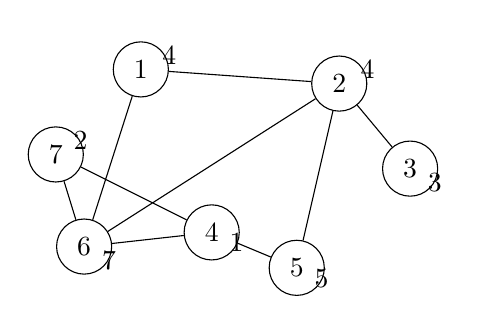
\begin{tikzpicture}[scale=0.9, every node/.style={circle,draw,minimum size=7mm,inner sep=0pt}]
  \node (1) at (1.4,2.8) {1};
  \node (2) at (4.2,2.6) {2};
  \node (3) at (5.2,1.4) {3};
  \node (4) at (2.4,0.5) {4};
  \node (5) at (3.6,0.0) {5};
  \node (6) at (0.6,0.3) {6};
  \node (7) at (0.2,1.6) {7};
  \draw (1)--(2) (1)--(6) (2)--(3) (2)--(5) (2)--(6)
        (4)--(5) (4)--(6) (4)--(7) (6)--(7);
  \node[draw=none] at (1.8,3.0) {\(4\)};
  \node[draw=none] at (4.6,2.8) {\(4\)};
  \node[draw=none] at (5.55,1.2) {\(3\)};
  \node[draw=none] at (2.75,0.35) {\(1\)};
  \node[draw=none] at (3.95,-0.15) {\(5\)};
  \node[draw=none] at (0.95,0.1) {\(7\)};
  \node[draw=none] at (0.55,1.8) {\(2\)};
\end{tikzpicture}
\end{center}

\begin{verbatim}
Sample Input
7 9 3
1 4
2 4
3 3
4 1
5 5
6 7
7 2
1 2
1 6
2 3
2 5
2 6
4 5
4 6
4 7
6 7
2000000000

Sample Output
7
2 1 6
2 2 3
3 4 5 7
\end{verbatim}

\paragraph{Cách chấm điểm.}
Đây là bài nộp đáp án. Với \(10\) tệp vào
\texttt{2/berry1.in} đến \texttt{2/berry10.in}, thí sinh nộp các tệp ra
\texttt{berry1.out} đến \texttt{berry10.out}. Nếu với một test, dòng đầu \(x\)
và phương án chia bên dưới không khớp, hoặc tệp ra sai định dạng, test đó
không có điểm. Có thể dùng công cụ \texttt{2/berry\_check} để kiểm tra; chỉ
khi công cụ in \texttt{Yes} thì đầu ra mới được xem là chấp nhận.

Với một đầu ra chấp nhận được, điểm được tính theo công thức trong đề:
\[
  \mathrm{score}=
  \left\lfloor
  10\exp\left(-\frac{2}{5}\left(\frac{d(\mathrm{best}-x)}
  {\mathrm{best}}\right)^2\right)
  \right\rfloor,
\]
trong đó \(d\) là hệ số chấm điểm ở dòng cuối dữ liệu vào, còn
\(\mathrm{best}\) là kết quả tối ưu của ban tổ chức. Chú ý: đầu ra chấp nhận
được chưa chắc có điểm.

Công cụ kiểm tra được gọi như sau:
\begin{verbatim}
2/berry_check <input-file> <output-file>
\end{verbatim}
Các thông báo gồm: \texttt{illegal exit} cho lỗi không rõ; \texttt{not connect}
khi một dòng chứa thành phần không liên thông; \texttt{duplicate} khi một điểm
được in hai lần; \texttt{extra} khi có dữ liệu thừa; \texttt{lack} khi tổng số
điểm không đúng; \texttt{answer not match} khi dòng đầu \(x\) không khớp kết
quả thực tế; và \texttt{Yes} khi đầu ra chấp nhận được.

Chương trình gốc xử lý dữ liệu dạng cây: sắp các đỉnh theo độ sâu, nhị phân
ngưỡng \(x\), rồi duyệt từ dưới lên để gom phần dư. Khi một phần dư đạt
ngưỡng, chương trình cắt ra một mảnh và ghi danh sách đỉnh; sau cùng in
phương án cho test được chọn.

\subsection{Chương trình 4: ghép theo ngưỡng biên}

Chương trình cuối trong phụ lục là cài đặt cho bài ghép cực đại--cực tiểu đã
phân tích ở phần chính. Nó đọc đồ thị hai phía có trọng số từ
\texttt{matching.in}, sắp xếp các trọng số cạnh, nhị phân ngưỡng \(\texttt{limit}\),
rồi ở mỗi ngưỡng chạy thủ tục ghép tăng đường để kiểm tra có thể ghép hết phía
trái hay không. Kết quả ngưỡng tốt nhất được ghi ra \texttt{matching.out}. Với
biến thể cực đại hóa cạnh nhỏ nhất, điều kiện giữ cạnh đổi chiều tương ứng như
đã nêu trong phần chính.

\end{document}
